\section{Theorie}
\label{sec:Theorie}

\subsection{Einleitung}
Ziel dieses Experiments ist es, gekoppelte Schwingkreise genauer zu untersuchen. 
Konkret soll hier das Verhalten der Energieverteilung auf die gekoppelten Systeme, sowie der Einfluss eines schwingenden 
Erregers auf den Schwingkreis ergründet werden.
Da elektromagnetische Schwingsysteme bei weitem einfacher zu vermessen sind als mechanische, werden die 
Messungen an ebensolchen durchgeführt. 
Die daraus gewonnen Erkenntnisse lassen sich problemlos auf andere gekoppelte Schwingsysteme übertragen. 

%%%%%%%%%%%%%%%%%%%%%%%%%%%%%%%%%%%%%%%%%%%%%%%%%%%%%%%%%%%%%%%%%%%%%%%%%%%%%%%%%%%%%%%%%%%%%%%%%%%%%%%%%%%%%%%%%%%%%%%
\subsection{Kapazitiv gekoppelte Schwingkreise, Eigenmoden, Schwebungen}
\begin{figure}
    \centering
    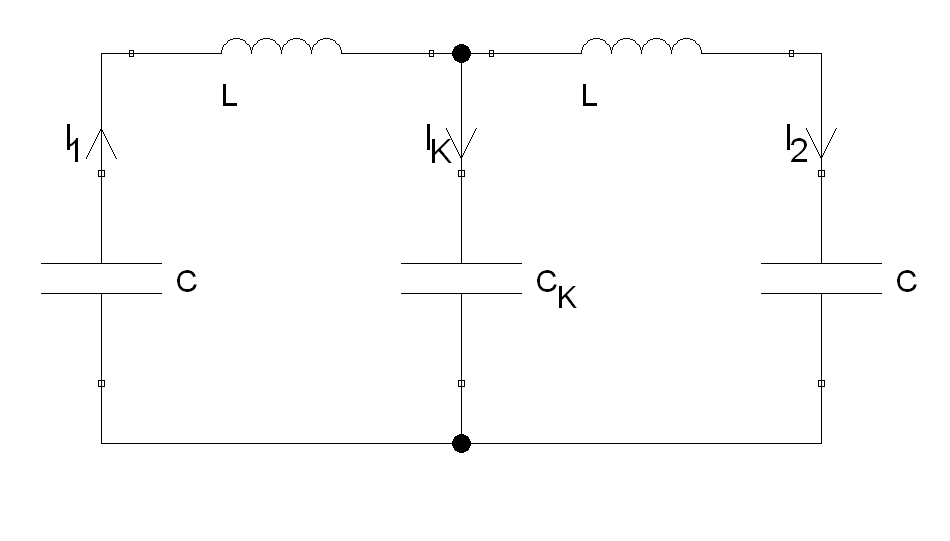
\includegraphics[width=0.75\textwidth]{plots/allg_gekopp_schwingkreis.png}
    \caption{Schaltbild eines kapazitiv gekoppelten Schwingkreises.}
    \label{fig:kap_gekopp}
\end{figure}
Die in \ref{fig:kap_gekopp} gezeigten Schwingkreise sind über einen Kondensator der Kapazität $C_K$ gekoppelt, wie es 
später auch im Experiment der Fall sein wird. 
Gemäß der Knotenregel (1. Kirchhoff'sches Gesetz) gilt die Beziehung
\begin{equation}
    I_1 = I_2 + I_K .
    \label{eqn:strom}
\end{equation}
Über die Maschenregel folgt für die über den Kondensatoren und Spulen abfallenden Spannungen 
\begin{align} %oder align, wenn gather nicht klappt 
    U_{C_1} + U_K = U_{L_1} 
    \label{eqn:masche1} \\
    U_{C_2} = U_{L_2} + U_K  
    \label{eqn:masche2} 
\end{align}
aus.
Mit der Definition der Kapazität ${C=\sfrac{Q}{U}}$, der Induktionsspannung ${U=- L \dot{I}}$ und \eqref{eqn:strom} folgt 
hierfür nach einmaligem zeitlichen Ableiten 
\begin{equation}
    \dot{Q} = I = C \dot{U} 
\end{equation}
\begin{align}
    \frac{1}{C} \dot{Q}_{C_1} + L \ddot{I}_{L_1} + \frac{1}{C_K} \dot{Q}_{K} \stackrel{\eqref{eqn:strom}}{=} 
    \frac{1}{C} I_1 + L \ddot{I_1} + \frac{1}{C_K} (I_1 - I_2) = 0 \label{eqn:dgl1} \\
    \frac{1}{C} \dot{Q}_{C_2} + L \ddot{I_2} - \frac{1}{C_K} \dot{Q}_{K} \stackrel{\eqref{eqn:strom}}{=}
    \frac{1}{C} I_2 + L \ddot{I_2} - \frac{1}{C_K} (I_1 - I_2) = 0 \label{eqn:dgl2}
\end{align}
Eine Möglichkeit zur Lösung der beiden gekoppelten Differentialgleichungen besteht darin, \eqref{eqn:dgl1} und \eqref{eqn:dgl2}
zu addieren und subtrahieren. So erhält man zwei voneinander entkoppelte Gleichungen der Variablen ${I_1 + I_2}$ und ${I_1 - I_2}$, 
die einfach mit einem harmonischen Ansatz gelöst werden können:
\begin{align}
    L (\ddot{I_1} + \ddot{I_2}) + \frac{1}{C} (I_1+I_2)=0 \label{eqn:prettydgl1} \\
    L (\ddot{I_1} - \ddot{I_2}) + (\frac{1}{C} + \frac{2}{C_K}) (I_1-I_2)=0 \label{eqn:prettydgl2}
\end{align}
Der harmonische Ansatz ${\ddot{x} = -\omega ^2 x}$ liefert mit den Kreisfrequenzen $\omega _+$ für \eqref{eqn:prettydgl1} 
und $\omega _-$ für \eqref{eqn:prettydgl2} die Lösungen 
\begin{align}
    (I_1+I_2)(t) &= A_+ \cos(\omega _+ t + \varphi _+) \quad \text{mit} \quad \omega _+ ^2= \frac{1}{LC} ,
    \label{eqn:add} \\
    (I_1-I_2)(t) &= A_- \cos(\omega _- t + \varphi _-) \quad \text{mit} \quad \omega _- ^2= \frac{1}{LC} + \frac{2}{LC_K} = \frac{C_K + 2C}{LCC_K} 
    \label{eqn:sub}
\end{align}
mit den Integrationskonstanten $A_+$, $A_-$, $\varphi _+$ und $\varphi _-$.
Die Schwingungsfrequenzen sind entsprechend $f_{\pm}=\sfrac{\omega _{\pm}}{2\pi}$.
Um die Lösungen für die ursprünglichen Ströme $I_1$ und $I_2$ zu erhalten, addiert und subtrahiert man \eqref{eqn:add} 
und \eqref{eqn:sub} erneut und dividiert durch zwei, sodass daraus 
\begin{align}
    I_1 (t) = \frac{1}{2} \bigl(A_+ \cos(\omega _+ t + \varphi _+) + A_- \cos(\omega _- t + \varphi _-)\bigr) \\
    I_2 (t) = \frac{1}{2} \bigl(A_+ \cos(\omega _+ t + \varphi _+) - A_- \cos(\omega _- t + \varphi _-)\bigr)
\end{align}
resultiert.

Jedes durch $N$ Systeme gekoppelte Schwingungssystem hat $N$ Fundamentalschwingungen -- auch bekannt unter Eigenmoden oder 
Normalschwingungen. 
Dies sind Schwingungen, die das System besonders \glqq bevorzugt\grqq{} ausführt. %deutsche Anführungszeichen
Allgemein besteht dann die Lösung für die Schwingung aus der Überlagerung der Eigenmoden, die durch Anfangsbedingungen 
festgelegt wird. 

In diesem Fall sind ${N=2}$ Systeme gekoppelt, die Eigenmoden sind durch ${I_1 + I_2}$ mit ${\omega _+}$ und ${I_1 - I_2}$ 
mit $\omega _-$ gegeben: 
Beginnt das System mit zwei gleichen Strömen ${I_1=I_2}$ zu schwingen, so gilt ${A_- = 0}$, sodass der Schwingkreis mit gleichen Strömen 
$I_1$ und $I_2$ mit der Frequenz ${f_+= \sfrac{\omega _+}{2\pi}}$, die ein einzelner LC-Kreis ebenfalls hätte, schwingt und gemäß 
\eqref{eqn:strom} kein Strom durch den Kopplungskondensator fließt. 
Dies ist die gleichphasige Normalschwingung -- die Ströme sind stets in Phase.
Wird das Gegenteil betrachtet, starten die Ströme $I_1=-I_2$ genau entgegengesetzt, oszilliert 
das System in der zweiten Eigenmode mit ${f_-=\sfrac{\omega _-}{2\pi} > f_+}$. 
Der Summenstrom $I_1 + I_2$ verschwindet und die Ströme schwingen genau gegenphasig. 
Selbsterklärend ist dies die gegenphasige Eigenschwingung. 

Ebenfalls zu betrachten sind sogenannte Schwebungen. 
In \ref{fig:kap_gekopp} kann eine beobachtet werden, wenn ${\omega _+ \approx \omega _-}$ gilt, also 
${C_K \gg C}$ ist. 
Startbedingungen sind, dass einer der beiden Ströme, beispielsweise $I_1$, anfangs von null verschieden ist und der 
jeweils andere Strom, gemäß dem Beispiel also $I_2$, in Ruhe ist, entsprechend keine Amplitude hat. 
Dann ergeben sich für die Ströme die Lösungen 
\begin{equation}
    I_1 (t) = \frac{A_+}{2} ( \cos(\omega _+ t + \varphi _+) + \cos(\omega _- t + \varphi _-))
    \label{eqn:ii1}
\end{equation}
und 
\begin{equation}
    I_2 (t) = \frac{A_+}{2} ( \cos(\omega _+ t + \varphi _+) - \cos(\omega _- t + \varphi _-)) .
    \label{eqn:ii2}
\end{equation}
Mit 
\begin{align}
    \tilde{\varphi}_+ &\coloneq \frac{\varphi _+ + \varphi _-}{2} ,
    & \tilde{\varphi}_- &\coloneq - \frac{\varphi _+ - \varphi _-}{2}
\end{align}
und den Additionstheoremen 
\begin{align}
    \cos x + \cos y &= 2 \cos(\frac{x+y}{2}) \cos(\frac{x-y}{2}) \\
    \cos x + \cos(y + \pi) &= \cos x - \cos y = 2 \cos(\frac{x+y}{2} + \frac{\pi}{2}) \cos(\frac{x-y}{2} - \frac{\pi}{2}) \\
        &=-2  \sin(\frac{x+y}{2}) \sin(\frac{x-y}{2})
\end{align}
lassen sich \ref{eqn:ii1} und \ref{eqn:ii2} zu 
\begin{gather}
    I_1 (t)= A_+ \cos(\frac{\omega _+ + \omega _-}{2}t +\tilde{\varphi}_+) \cos(\frac{\omega _+ - \omega _-}{2}t -\tilde{\varphi}_+) \\
    I_2 (t)=-A_+ \sin(\frac{\omega _+ + \omega _-}{2}t +\tilde{\varphi}_+) \sin(\frac{\omega _+ - \omega _-}{2}t -\tilde{\varphi}_+)
\end{gather}
umformen.
Es ist zu erkennen, dass die Ströme mit der Frequenz 
\begin{equation}
    \omega _\text{Schwingung} = \frac{\omega _+ + \omega _-}{2} \approx \omega _+
\end{equation}
oszillieren, dass die Amplitude jedoch mit der bei weitem geringeren Frequenz 
\begin{equation}
    \omega _\text{Amplitude} = \frac{\omega _+ - \omega _-}{2} \ll \omega _+
\end{equation} 
ebenfalls eine Oszillation aufweist. 
Das Doppelte der dazugehörigen Frequenz nennt sich Schwebungsfrequenz und ist 
\begin{equation}
    f_\text{Schwebung}= \frac{\omega _\text{Amplitude}}{\pi}=\frac{\omega _+ - \omega _-}{2 \pi}.
\end{equation} 
Sie gibt an, wie schnell die Energie zwischen den beiden Schwingungssystemen hin- und herpendelt. 
Werden nämlich die Schiwngungen der Amplituden betrachtet -- also die Schwingungen mit $\omega _\text{Amplitude}$ --, 
ist zu erkennen, dass die von $I_1$ jeweils gegenphasig zu $I_2$ oszilliert. 
Dies indiziert den besagten Energieaustausch. 
\FloatBarrier

%%%%%%%%%%%%%%%%%%%%%%%%%%%%%%%%%%%%%%%%%%%%%%%%%%%%%%%%%%%%%%%%%%%%%%%%%%%%%%%%%%%%%%%%%%%%%%%%%%%%%%%%%%%%%%%%%%%%%%%%%
\subsection{Erzwungene Schwingungen des gekoppelten Schwingkreises}
%%%%%%
%%HIER ein Schaltbild wie in Abb. 4 einfügen
%%%%%%
\begin{figure}
    \centering
    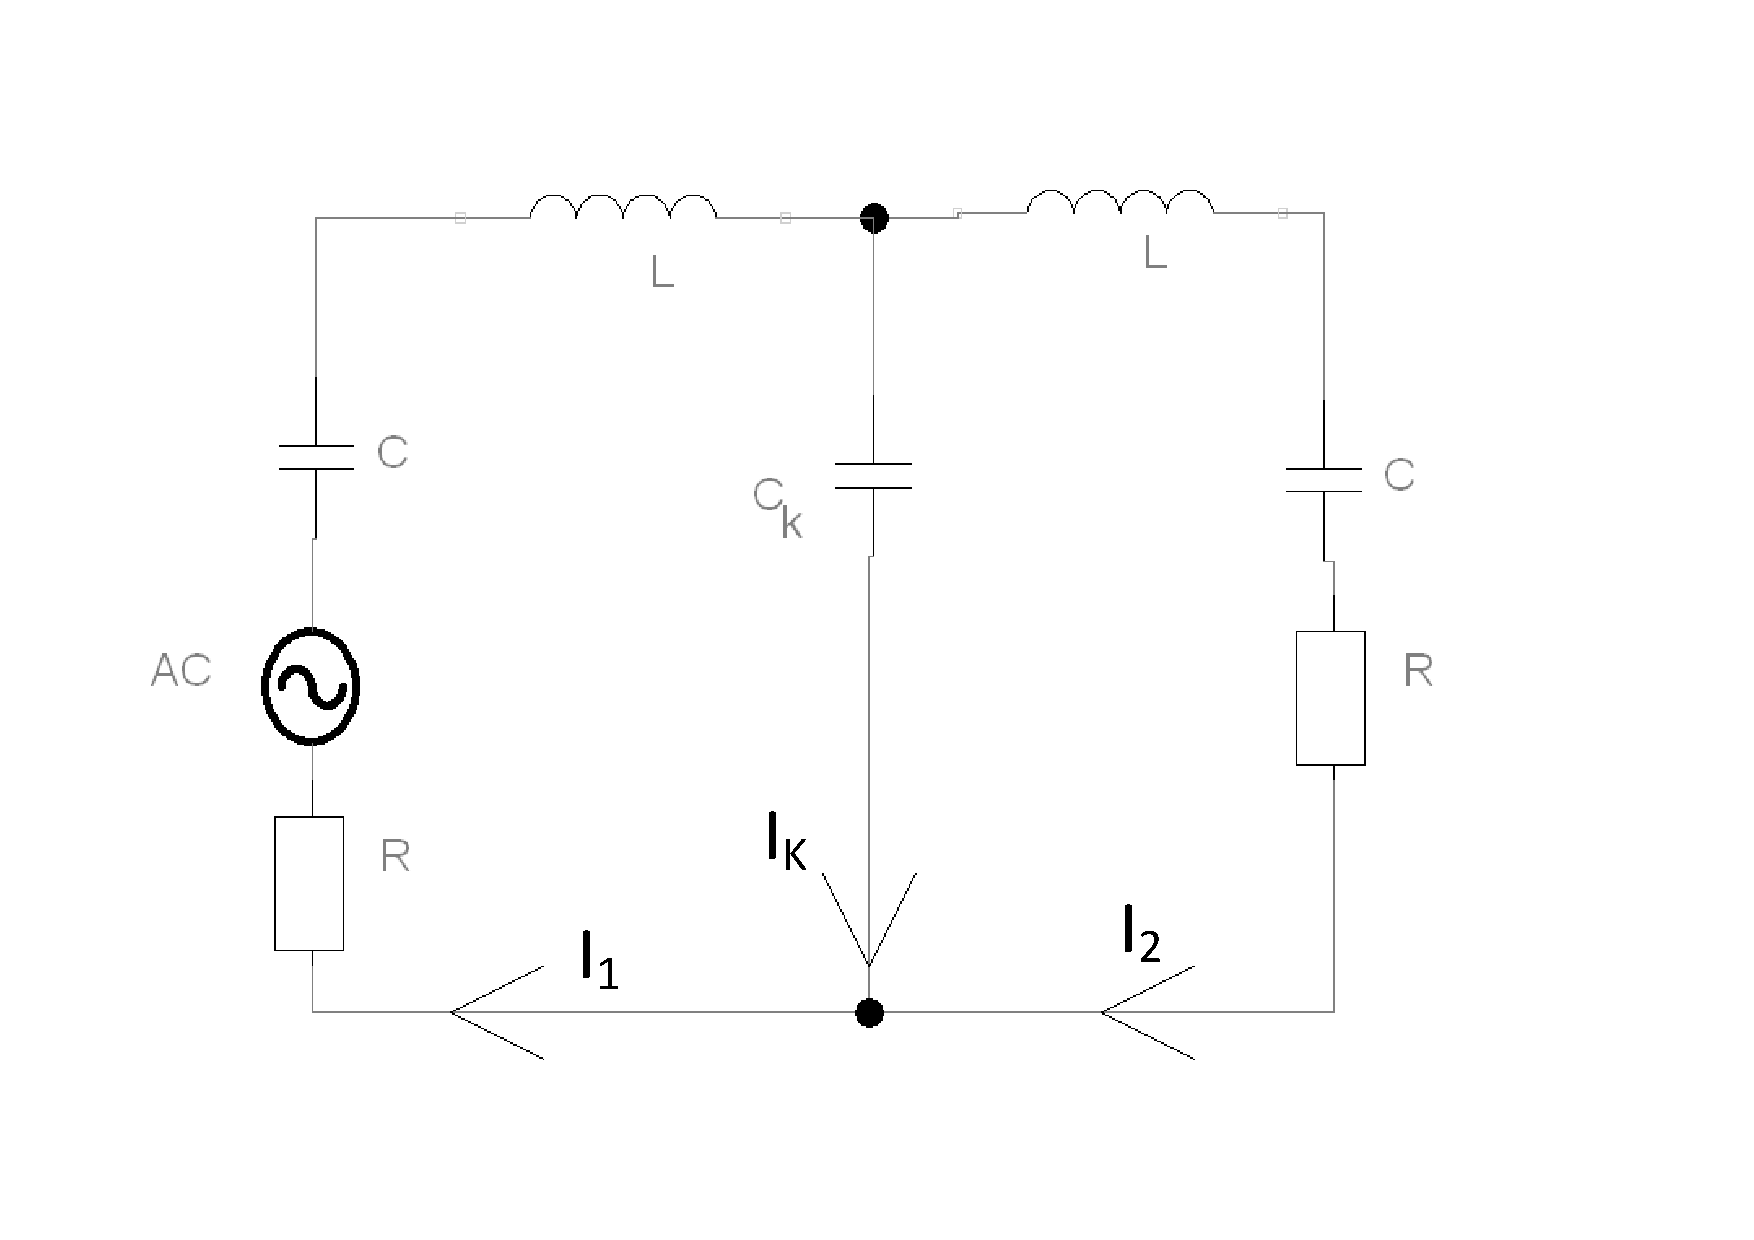
\includegraphics[width=0.75\textwidth]{plots/gekop_schw_kreis1.pdf}
    \caption{Durch einen Sinusgenerator erzwungene Schwingungen mit verlustbehafteten Größen.}
    \label{fig:gezwung-sinus}
\end{figure}
Wird ein Sinusgenerator mit ${\tilde{U}(t)=U_0 \symup{e}^{\symup{i}\omega t}}$ gemäß Abbildung \ref{fig:gezwung-sinus} in den Schaltkreis 
eingebunden, und werden Verlustwiderstände als ohmsche Widerstände jeweils berücksichtigt, ergeben sich mit den Kirchhoff'schen 
Gesetzen die Zusammenhänge 
\begin{gather}
    \tilde{U}=(\frac{1}{\symup{i}\omega C} +  \symup{i} \omega L + \frac{1}{\symup{i}\omega C_K} + R)I_1 - \frac{1}{\symup{i}\omega C_K} I_2 \\
    \text{und} \quad (\symup{i}\omega L + \frac{1}{\symup{i}\omega C} + R+ \frac{1}{\symup{i}\omega C_K}) I_2 - \frac{1}{\symup{i}\omega C_K}I_1 =0 \text{.}
\end{gather}
Nach einigen Umformungen kann ein betragsmäßiges Verhältnis von $I_2$ und $\tilde{U}$ aufgestellt werden, wobei eine Impedanz ${Z(\omega)}$ 
der Übersicht halber mit 
\begin{equation*}
    Z(\omega) = \omega L - \frac{1}{\omega} (\frac{1}{C} + \frac{1}{C_K})    
\end{equation*}
definiert wird:
\begin{gather}
    \lvert I_2 \rvert = \lvert \Omega \rvert \lvert \tilde{U} \rvert \\  \\
    \text{mit} \quad \Omega = \Biggl(\sqrt{4 \omega ^2 C_K^2 R^2 Z(\omega)^2 + (\frac{1}{\omega C_K} - \omega C_K Z(\omega)^2 + \omega R^2 C_K)^2 }\Biggr)^{-1} .
\end{gather}
Dabei stellt $\Omega (\omega)$ den sogenannten Leitwert dar. 
Dieser geht jeweils für ${\omega \to 0}$ und ${\omega \to \infty }$ gegen Null und hat zwei Maxima für ${\omega = \omega _+}$ und 
${\omega = \omega _-}$. 
In diesen Fällen gilt:
\begin{align}
    \Omega (\omega _+) &= \frac{1}{R\sqrt{4 + \frac{R^2C_K^2}{LC}}} \approx \frac{1}{2R} \\
    \Omega (\omega _-) &= \frac{1}{R\sqrt{4 + \frac{R^2C_K^2}{LC}(1 + \frac{C}{C_K}})} \approx \frac{1}{2R}  
\end{align}
Die Näherungen ergeben sich dadurch, dass Werte der üblichen Größenordnungen für die Widerstände eingesetzt werden.
Daraus wird ersichtlich, dass der zweite Summand unter der Wurzel im Vergleich zur $4$ unbedeutend klein ist. 

